\def\beginanswers{\iffalse}
%%\def\beginanswers{\iftrue}

\documentclass[10pt]{article}
\usepackage{amsmath,amsfonts,amsthm,amssymb}
\usepackage{graphicx}
\usepackage{enumerate}
\usepackage{upquote,textcomp}
\usepackage{listings}
\usepackage{color}

\definecolor{mygreen}{rgb}{0,0.6,0}
\definecolor{mygray}{rgb}{0.5,0.5,0.5}
\definecolor{mymauve}{rgb}{0.58,0,0.82}


\lstset{frame=tb,
  language=,
  aboveskip=3mm,
  belowskip=3mm,
  showstringspaces=false,
  columns=flexible,
  keepspaces=true,
  basicstyle={\small\ttfamily},
  numbers=none,
  numberstyle=\tiny\color{black},
  keywordstyle=\color{black},
  commentstyle=\color{black},
  stringstyle=\color{black},
  breaklines=true,
  breakatwhitespace=true,
  tabsize=3
}

\lstset{frame=tb,
  language=Python,
  aboveskip=3mm,
  belowskip=3mm,
  showstringspaces=false,
  columns=flexible,
  basicstyle={\small\ttfamily},
  numbers=none,
  numberstyle=\tiny\color{mygray},
  keywordstyle=\color{blue},
  commentstyle=\color{mygreen},
  stringstyle=\color{mymauve},
  breaklines=true,
  breakatwhitespace=true,
  tabsize=3
}


\newcommand{\vect}[1]{{\bf #1}}                 %for bold chars
\newcommand{\vecg}[1]{\mbox{\boldmath $ #1 $}}  %for bold greek chars
\newcommand{\matx}[1]{{\bf #1}}

\setlength{\parindent}{0in}
\setlength{\parskip}{1em}
\setlength{\textheight}{9.5in}
\setlength{\textwidth}{7in}
\setlength{\headsep}{0in}        % distance from top of page to address
\setlength{\topmargin}{-0.5in}
\setlength{\oddsidemargin}{-0.5in}
\setlength{\evensidemargin}{-0.5in}


\begin{document}
\thispagestyle{empty}

\vspace*{0.5in}

\begin{center}
\Large
\textbf{Open Source Software --- CSCI-4961-01 --- Summer 2018} \\
\textbf{Quiz 2} \\
\textbf{August 16, 2018}
\end{center}


%%%%%%%%%%%%%%%%%%%%%%%%%%%%%%%%%%%%%%%%%%%%%%%%%%%%%%%%%%%%%%%%%%%%%%%%
%%%%%%%%%%%%%%%%%%%%%%%%%%%%%%%%%%%%%%%%%%%%%%%%%%%%%%%%%%%%%%%%%%%%%%%%
\beginanswers
\begin{center}
\Large
\textbf{SOLUTIONS}
\end{center}

%%%%%%%%%%%%%%%%%%%%%%%%%%%%%%%%%%%%%%%%%%%%%%%%%%%%%%%%%%%%%%%%%%%%%%%%
\else
%%%%%%%%%%%%%%%%%%%%%%%%%%%%%%%%%%%%%%%%%%%%%%%%%%%%%%%%%%%%%%%%%%%%%%%%


\begin{center}

\textbf{\Large Name:} \underline {\hspace{2.0in}} \\

\bigskip
\bigskip

\centerline{
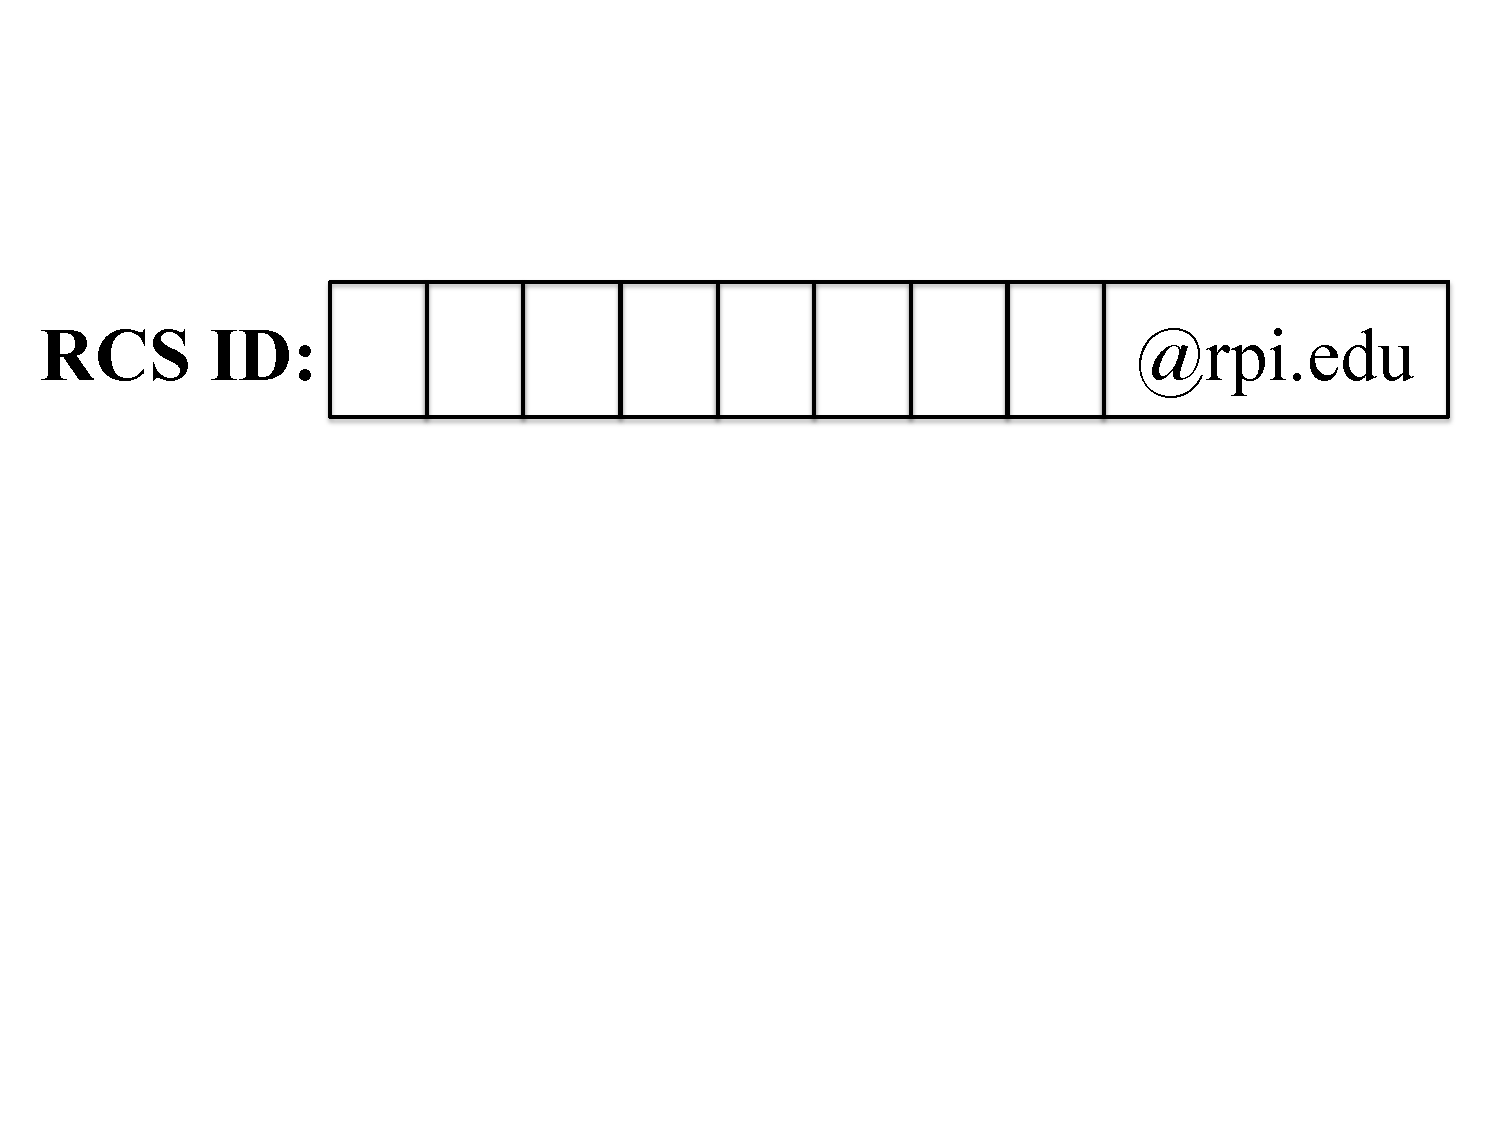
\includegraphics[height=0.5in]{boxes}
}

%%  \begin{tabular}{|p{0.1in}|p{0.1in}|p{0.1in}|p{0.1in}|p{0.1in}|p{0.1in}|p{0.1in}|p{0.1in}|l|}
%%    \hline \\
%%   & & & & & & & & \textbf{\large @rpi.edu} \\
%%  \hline
%%  \end{tabular} 
%%  
%%  \end{tabular}

\bigskip

\textbf{\Large RIN\#:} \underline {\hspace{1.5in}}  

\vspace*{0.4in}
{\large\bf Honor pledge: On my honor I have neither given
nor received aid on this exam.}

\vspace*{0.1in}
{\large\bf Please sign here to indicate that you agree with the honor pledge: \underline {\hspace{1.5in}}}
\end{center}

\vspace*{.45in} 

{\large\bf Instructions:}
\begin{itemize}
\item You have 90 minutes to complete this test.
\item Clearly print your name, RCS ID (in all caps.) and your RIN at the top of your exam.
\item This test is open book, open notes and open computer. You {\textbf may not} use the internet. Please turn off your wifi.
\item There are \textbf{6 questions} on this test worth a total of
  \textbf{104 points}.
\end{itemize}


\newpage

%%%%%%%%%%%%%%%%%%%%%%%%%%%%%%%%%%%%%%%%%%%%%%%%%%%%%%%%%%%%%%%%%%%%%%%%
\fi
%%%%%%%%%%%%%%%%%%%%%%%%%%%%%%%%%%%%%%%%%%%%%%%%%%%%%%%%%%%%%%%%%%%%%%%%

\begin{enumerate}

\item Short answers (38 pts)

    \begin{enumerate}
    \item There are numerous fields in which Scientific Computing is essetntial. In class, we defined 16.  Give 4 of the fields we called out. (8 pts)

    \beginanswers
        \begin{itemize}
        \item Finite Element Modeling - Structural Safety
        \item Fluid Mechanics - Aerodynamics - Aircraft Design
        \item Circuit Simulation
        \item Genomics and Drug Simulation
        \item Image Processing Applications
        \item Airline Scheduling, Linear and Nonlinear Programming Application
        \item Astronomy and Space Computations
        \item Simulation of Materials
        \item Manufacturing Process
        \item Network Simulation
        \item Weapon Simulation/Modeling
        \item Solving NP-hard/complete Problems
        \item Protein Folding
        \item SETI, Milkyway@Home
        \item Physics Engines for Game Playing
        \item Chemistry
        \end{itemize}
    \else
	\begin{enumerate}
	\item 
	\bigskip
	\bigskip
	\item
	\bigskip
	\bigskip
	\item 
	\bigskip
	\bigskip
	\item
	\bigskip
	\bigskip
        \end{enumerate}
    \fi
    \bigskip
    \bigskip

    \item Looking at the Angry Birds Game, answer the following two questions. (4 pts)
	\begin{enumerate}
	\item Which module encapsulates the physics of the simulation?:
	    \beginanswers
	        \begin{itemize}
		\item pymunk
		\end{itemize}
	    \else
            \bigskip
            \bigskip
            \bigskip
            \bigskip
            \fi
        \item The entirety of the physics simulation for a given time step is contained in a single call. What is the call to advance the simulation one step?:
	    \beginanswers
                \begin{itemize}
                \item space.step(dt) 
		\end{itemize}
            \else
            \bigskip
            \bigskip
            \bigskip
            \bigskip
	    \fi
	\end{enumerate}
    \bigskip
    \bigskip
    \item From our notes, name 3 statistical  languages with a BSD based license (6 points):
        \beginanswers
            \begin{itemize}
	    \item SciPy
	    \item Panda
	    \item Shogun
            \end{itemize}
        \else
            \begin{enumerate}
	    \item 
	    \bigskip
	    \bigskip
	    \item
	    \bigskip
	    \bigskip
	    \item 
	    \bigskip
	    \bigskip
            \end{enumerate}
        \fi
    \bigskip
    \bigskip
    \item From our notes, name four benefits of incremental testing (8 points):
        \beginanswers
            \begin{itemize}
	    \item Errors easier to isolate, find, fix reduces developer bug-fixing load
	    \item System is always in a relatively working state - good for developers and customers.
	    \item System complexity can be understood incrementally.
	    \item Users can develop a better understanding of their requirements.
            \end{itemize}
        \else
            \begin{enumerate}
	    \item 
	    \bigskip
	    \bigskip
	    \item
	    \bigskip
	    \bigskip
	    \item 
	    \bigskip
	    \bigskip
	    \item 
            \bigskip
            \bigskip
            \end{enumerate}
        \fi
    \bigskip
    \bigskip
    \item From our notes, name what percent of open source projects have a single developer (as of 2013). Any answer within 5 points of the correct solution will be accepted. (2 points)]?
        \beginanswers
            \begin{itemize}
	    \item 51%
            \end{itemize}
        \else
            \begin{enumerate}
	    \item
	    \bigskip
	    \bigskip
            \end{enumerate}
        \fi
    \bigskip
    \bigskip
    \item From our notes, name three governance models (6 points):
        \beginanswers
            \begin{itemize}
	    \item Benevolent dictator
	    \item Meritocracy
	    \item Dr. Who Rengeneration Model
            \end{itemize}
        \else
            \begin{enumerate}
	    \item 
	    \bigskip
	    \bigskip
	    \item
	    \bigskip
	    \bigskip
	    \item 
	    \bigskip
	    \bigskip
            \end{enumerate}
        \fi
    \bigskip
    \bigskip
    \item Who \verb|"owns"| an open source project? (4 points)
        \beginanswers
            \begin{itemize}
	    \item Who: No one
	    \item Why: Forking
	    \end{itemize}
        \else
            \begin{enumerate}
	    \item (Who:)
	    \bigskip
	    \bigskip
	    \item (Why:)
	    \bigskip
	    \bigskip
	    \end{enumerate}
        \fi
    \end{enumerate}

\newpage

\item \textit{Scientific Computation} Feel free to review, edit or run code from the Scientific Computation lecture or lab to answer the following questions. (16 pts):

\textit{Note:} If you import \verb|networkx| into python and issue the command \verb|help(networkx.shortest_path)| it will provide you with additional information on the shortest path algorithm. In particular, notice that if you do not provide a target, then the algorithm returns a dictionary where the keys are words that can be reached from the source and the values are the list of nodes. This information will help you with this question.

    \begin{enumerate}
    \item Consider your word ladder code to find the shortest path from one five letter word to another.
	\begin{enumerate}
	\item Assuming that you are not allowed to change the order of the letters, what is the length of the longest, shortest path from the word \textit{party}? (4 points)
	    \beginanswers
		\begin{itemize}
		\item 18
		\end{itemize}
	    \else
	    \bigskip
	    \bigskip
	    \bigskip
	    \bigskip
	    \fi
        \item What is the final word in the path? (4 points)
	    \beginanswers
		\begin{itemize}
		\item amigo
		\end{itemize}
	    \else
	    \bigskip
	    \bigskip
	    \bigskip
	    \bigskip
            \fi
	\end{enumerate}

    \item Now consider the degree of a word as the number of other words that can be made from it by changing a single letter and keeping the word order the same. 
        \begin{enumerate}
	\item What words have the maximum degree of 25? (4 points)
	    \beginanswers
	        \begin{itemize}
		\item cores, bares
	        \end{itemize}
	    \else
	    \bigskip
	    \bigskip
	    \bigskip
	    \bigskip
	    \fi
	\item There are far more words with degree 0. How many are there? (4 points)
	    \beginanswers
	        \begin{itemize}
		\item 671
	        \end{itemize}
	    \else
	    \bigskip
	    \bigskip
	    \bigskip
	    \bigskip
	    \fi
	\end{enumerate}	
    \end{enumerate}

\newpage

\item \textit{Statistical Computation} Feel free to review, edit or run code from the Statistical Computation lecture or lab to answer the following questions. (10 pts):
    \begin{enumerate}
    \item Consider the topmovie data we used in our \textit{R} examples. 
	\begin{enumerate}
	\item What is the Minimum, 1st Quartile, Median, Mean, 3rd Quartile, and Maximum values for the box office? (4 points)
	    \beginanswers
		\begin{itemize}
		\item 52.58, 70.28, 93.60, 117.47, 134.62, 759.56
		\end{itemize}
	    \else
	    \bigskip
	    \bigskip
	    \bigskip
	    \bigskip
	    \fi
	\item If we want to look at the relationship between the box office and the year, how would we generate a scatterplot with year on the \textit{X-axis} and box office on the \textit{Y-axis}? Type the command below: (6 points)
            \beginanswers
		\begin{itemize}
		\item plot(topmovies$year, topmovies$box)
		\end{itemize}
	    \else
	    \bigskip
	    \bigskip
	    \bigskip
	    \bigskip
	    \fi
	\end{enumerate}
    \end{enumerate}

\newpage


\item \texttt{Testing and Continuous Integration} Feel free to review, edit or run code from the Testing and Continuous Integration lecture or lab to answer the following questions. (15 pts):
\bigskip

Consider the following Python module implementing the merge\_sort algorithm:
\begin{verbatim}
import random

def merge(L1, L2):
  """
  Assume L1 and L2 are sorted.
  Create a new list L that is the merged
  version of L1&L2.
  """
  L = []
  i = 0
  j = 0
  while i < len(L1) and j < len(L2):
    if L1[i] < L2[j]:
      val = L1[i]
      L.append( val )
      i += 1
    else:
      val = L2[j]
      L.append( val )
      j += 1
  ## at this point, either L1 or L2 has run out of values
  ## add all the remaining values to the end of L.
  L.extend(L1[i:]) 
  L.extend(L2[j:])
  return L

def merge_sort_recursive(L):
  """ 
  Complexity: O(n logn)
  The function calls itself recursively logn times,
  and each time about n elements are merged.
  """
  if len(L) <= 1:
    return L

  length = len(L)
  mid = length // 2
  left = merge_sort_recursive(L[:mid])
  right = merge_sort_recursive(L[mid:])
  return merge(left,  right)

if __name__ == "__main__":
  ##Testing code
  k = 10
  L = list(range(k))
  random.shuffle(L)
  print("Before:", L)
  L = merge_sort_recursive(L)
  print("After:", L)
\end{verbatim}

\newpage

Generate a python file, \textit{test\_merge.py} that uses the unittest framework to thoroughly test the \textit{merge} and \textit{merge\_sort\_recursive} functions. 
Assume \textit{white box} testing. 
You should be able to come up with at least 3 test cases for \textit{merge} and at least 2 test cases for \textit{merge\_sort\_recursive}
    \beginanswers
\begin{verbatim}
import unittest
import merge_sort

class TestMS(unittest.TestCase):

  def setUp(self):
    pass

  def test_merge_1(self):
    L1 = list(range(0, 10, 2))
    L2 = list(range(1, 10, 2))
    ans = list(range(10))

  def test_merge_2(self):
    L1 = list(range(0, 10))
    L2 = []
    ans = list(range(10))
    self.assertEqual( merge_sort.merge(L1, L2), ans)

  def test_merge_3(self):
    L1 = list(range(0, 10))
    L2 = []
    ans = list(range(10))
    self.assertEqual( merge_sort.merge(L2, L1), ans)

  def test_merge_4(self):
    self.assertEqual( merge_sort.merge_sort_recursive([]), [])

  def test_merge_5(self):
    self.assertEqual( merge_sort.merge_sort_recursive(list(range(9, -1, -1))), list(range(10)))

  def test_merge_6(self):
    self.assertEqual( merge_sort.merge_sort_recursive([1, 4, 2, 0]), [0, 1, 2, 4])

if __name__ == '__main__':
  unittest.main()
\end{verbatim}
    \else
    Write your \textit{test\_merge.py} function in the space below:

    \hspace*{-0.4in}\framebox(540,600){}
    \fi

\newpage

\item \texttt{MongDB} Feel free to review, edit or run code from the MongoDB lecture or lab to answer the following questions. (15 pts):

	Consider the definitions file we used for our MongoDB lab, particularly for \textit{checkpoint4.py} and \textit{checkpoint5.py}. 
	\begin{enumerate}
	\item Write the sequence of commands to reset the database to the contents of the file \verb|definitions.json|. Use \verb|$| to indicate commands typed on the command line and \verb|>| to indicate commands typed into the mongo prompt. You should assume that the database is already in mongodb with the name \verb|mongo_db_lab|, i.e. (3 points)
	\begin{verbatim}
	$ mongo
	MongoDB shell version v4.0.0
	connecting to: mongodb://127.0.0.1:27017
	MongoDB server version: 4.0.0
	> show dbs
	admin         0.000GB
	config        0.000GB
	local         0.000GB
	mongo_db_lab  0.000GB
	> quit()
	$
	\end{verbatim}

\beginanswers

\begin{verbatim}
$ mongo
MongoDB shell version v4.0.0
connecting to: mongodb://127.0.0.1:27017
MongoDB server version: 4.0.0
> use mongo_db_lab
switched to db mongo_db_lab
> db.definitions.drop()
true
> quit()
ubuntu@eec278129a30:~/mongodb_lab$ mongoimport --host=127.0.0.1 --db mongo_db_lab --collection definitions --file definitions.json
2018-08-15T16:21:34.169+0000	connected to: 127.0.0.1
2018-08-15T16:21:34.205+0000	imported 147 documents
ubuntu@eec278129a30:~/mongodb_lab$ 
\end{verbatim}

\else
Write your commands in the space below:


\hspace*{-0.4in}\framebox(540,400){}
\fi

\newpage
\item How many entries in the database have the string \verb|" RPI "| in them? (2 points)
\beginanswers
\bigskip
13
\bigskip
\else
\bigskip
\bigskip
\bigskip
\fi

\item Now write Python code to search through the database, replace every occurrence of \verb|" RPI "| in a definition with \verb|" Rensselaer Polytechnic Institute "|, and write the modified records back out to the database. Be careful with the search and replacement strings. You do not want to change the string \verb|"(RPI)"|. (Also, if you are testing your code make sure that you reset your database before running.) (10 points)

\beginanswers
\begin{verbatim}
from pymongo import MongoClient

client = MongoClient()

if __name__ == '__main__':
  db = client.mongo_db_lab
  collection = db.definitions

  # All records
  all_documents = list(collection.find())

  print(len(all_documents))
  found = 0
  ids = []
  for document in all_documents:
    if ' RPI ' in document['definition']:
      document['definition'] = document['definition'].replace(' RPI ', ' Rensselaer Polytechnic Institute ')
      collection.update({'_id':document['_id']}, document)
      ids.append(document['_id'])
      found += 1

  print(found)
  for id in ids:
    print(collection.find({'_id': id})[0])
\end{verbatim}
\else
Write your code in the space below:


\hspace*{-0.4in}\framebox(540,500){}
\fi
\newpage
\end{enumerate}


\item \texttt{Virtualization and Containers} Feel free to review, edit or run code from the Virtualization and Containers lecture or lab to answer the following questions. (10 pts):

\begin{enumerate}
	\item Look at the following command to run a docker instance. 
	
	\verb|$ docker run -i -t -p 8888:8888 ubuntu:latest|
	
	Briefly describe what the following parts of the line do to the execution: (5 points)
	\begin{enumerate}
	\beginanswers
		\item -i:
		Run in interactive mode
		\bigskip
		\item -t:
		Allocate a pseudo-TTY
		\bigskip
		\item -p 8888:7777
		publish container port 7777 to host port 8888  
		\bigskip
		\item ubuntu
        Image to be run
		\bigskip
		\item :latest
		Version (tag) to run on the selected image
		\bigskip		
	\else	
		\item -i:
		\bigskip
		\bigskip
		\item -t:
        \bigskip
        \bigskip
		\item -p 8888:7777
        \bigskip
        \bigskip
        \item ubuntu
        \bigskip
        \bigskip
        \item :latest
        \bigskip
        \bigskip		
	\fi
    \end{enumerate}
 \item Assume you have the Dockerfile below:
 \begin{verbatim}
 # Comments in Dockerfiles
 FROM ubuntu:latest
 
 RUN apt-get update
 RUN apt-get install sudo
 RUN apt-get --yes install apt-transport-https
 RUN apt-get --yes install dbus
 RUN apt-get --yes install python3
 RUN apt-get install python3-pip
 
 RUN mkdir -p /data/db
 
 RUN useradd -d /home/ubuntu -ms /bin/bash -g root -G sudo ubuntu
 RUN echo "root:Docker!" | chpasswd
 RUN echo "ubuntu:ubuntu" | chpasswd
 
 USER ubuntu
 WORKDIR /home/ubuntu
\end{verbatim}
\begin{enumerate}
	\beginanswers
	\item Write the command to compile this docker file into an image with the name profsfavorites (Assume the Dockerfile is in the current directory) (2 points):
	\begin{verbatim}
	> docker build -t profsfavorites . 
	\end{verbatim}
	\bigskip
	\item What commands would be added to the Dockerfile to install \verb|git| and \verb|vim| (both are available through apt-get) (2 points)?
	\begin{verbatim}
	RUN apt-get --yes install git
	RUN apt-get --yes install vim
	\end{verbatim}
	\bigskip
	\item How many user accounts are there on the machine (do not count the root account) (1 point)?
	\begin{verbatim}
	1 - ubuntu
		\end{verbatim}
\bigskip
\else
	\item Write the command to compile this docker file into an image with the name profsfavorites (2 points):
	\bigskip
	\bigskip
	\item What commands would be added to the Dockerfile to install \verb|git| and \verb|vim| (both are available through apt-get) (2 points)?
	\bigskip
	\bigskip
	\item How many user accounts are there on the machine (do not count the root account) (1 point)?
	\bigskip
	\bigskip
	\fi
\end{enumerate}
\end{enumerate}


\end{enumerate}
\end{document}

